\runningheader{Oppgave d)}{}{Side \thepage\ av \numpages}

% ********************************************************
% oppgave d) 
% ********************************************************  
\item
  Lag følgende modell.
  \begin{figure}[H]
    \centering
    \hspace*{0mm}\scalebox{0.8}{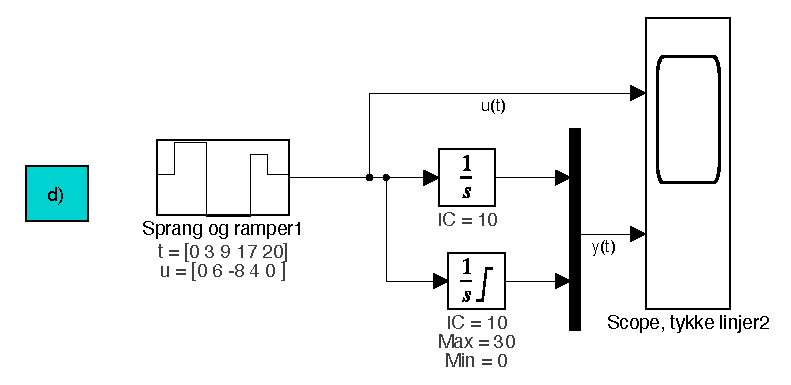
\includegraphics{2d.pdf}}
  \end{figure}
 Signalet $u(t)$ er modellert med {\sf Sprang og
    ramper}-blokken med følgende verdier
  \begin{itemize}
  \item   {\sf Tidspunkter} som {\tt [0~3~9~17~20]}
    \item {\sf Utgangsverdier} som {\tt [0~6~-8~-4~0]} 
  \end{itemize}
  som betyr at
 \begin{equation}
    u(t) =
 \begin{cases}%
  0 & \text{for } 0 \leq t< 3\\
   6  & \text{for } 3 \leq t <9 \\
   -8  &  \text{for }9 \leq t <17 \\
   4  & \text{for } 17 \leq t <20 \\
   0  & \text{for } t \geq 20 
 \end{cases}
  \end{equation}
  Velg interpolasjonsmetode som \dbox{\tt Trappetrinn} fra
    rullegardinmenyen i blokken.  
    Den svarte avlange blokken er en {\sf Mux} som multiplekser flere signal
  inn i samme ``ledning''. Den summerer altså ikke signalene. 
  I blokken {\sf Integrator med begrensing} er
  utgangen begrenset nedad til $y_{min}{=}0$ og oppad til $y_{max}{=}30$. 
   Begge integratorene har  initialverdi $y(0){=}10$. 
  {\color{red}La simuleringstiden fortsatt være 25 sekund.}


  
    {\bf Svar på følgende spørsmål:    }
  
  \begin{enumerate}[label=d\arabic*)]
  \item    Simuler modellen og ta med simuleringsresulatet
    i innleveringen.

\item Forklar med ord hva simuleringsresulatet viser. Forklar først
  den blå kurven, og deretter den røde kurven.

\item Hvordan ville du prinsipielt implementert
      integratorbegrensing i kode?

\item Forklar hva som skjer dersom du prøver å sette initialverdien
  til 40 i \\ {\sf Integrator med begrensing}-blokken?

\item   Hvorfor beholder  $y(t)$ sin verdi når $u(t)$ går
  til 0 fra $t{>}20$~sekund? Hva er den intuitive forklaringen?

\end{enumerate}

  {\color{blue}Vær klar over at du kan skrive både matematiske
    uttrykk,  kommentarer, funksjoner og kode i
  alle feltene i alle Simulink-blokkene. Under vises noen eksempler på hva du kan
  skrive i feltet  {\sf Utgangsverdier}:
  \begin{itemize}
    \setlength\itemsep{0mm}
  \item  {\tt [0~4~0~-5~2]*0.1}
  \item  {\tt [0~-3~2~0~1]  \hspace*{3mm} \%[0~4~0~-5~2] } 
  \item  {\tt randn(1,5)}
  \item  {\tt 1:0.1:1.4}
  \end{itemize}
  Uansett hvilke tall du skriver, så må alltid antall elementer i
  {\sf  Tidspunkter} og {\sf Utgangsverdier} være likt.
}
